\documentclass[]{article}

\usepackage[within=section]{newfloat}
\usepackage{caption}
\usepackage{url}
\usepackage{graphicx}

\DeclareFloatingEnvironment[name=کد,within=none,placement=h]{code}
\captionsetup{belowskip=0pt,aboveskip=0pt}

\usepackage{xcolor}
\usepackage[section,newfloat=true]{minted}

\usemintedstyle{manni}

\definecolor{mintedbackground}{rgb}{0.95,0.95,0.95}
\setminted[python]{linenos,breaklines,bgcolor=mintedbackground,frame=leftline,autogobble}
\setminted[bash]{breaklines,bgcolor=mintedbackground,frame=leftline,autogobble}

\usepackage{enumerate}

\usepackage{xepersian}
\settextfont{XB Niloofar}


% Title Page
\title{گزارش پیاده‌سازی الگوریتم‌های \\ \lr{Logistic Regression} \\ و \\ \lr{‌Softmax}}
\author{محمد شعاعی\\ \and امیر محمد مزارعی}
\begin{document}
\maketitle
	
\part{توابع و کلاس‌ها}
برای هر کدام از قسمت‌های مورد نیاز یک کلاس جدا پیاده سازی شده است. کلاس ها و متدهای مربوط به هر کلاس به شرح زیر است:
\begin{enumerate}
	\item \lr{\mintinline{python}{BinaryClassifier(eta, tol, n_iters)}}: این کلاس پیاده سازی \lr{classification} دو کلاسه است که شامل متد‌های زیر است:
	\begin{itemize}
		\item \lr{\mintinline{python}{fit(X, y)}}
		\item \lr{\mintinline{python}{predict(X)}}
		\item \lr{\mintinline{python}{predict_proba(X)}}
		\item \lr{\mintinline{python}{cost(X, y)}}
		\item \lr{\mintinline{python}{sigmoid(z)}}
	\end{itemize}
	\item \lr{\mintinline{python}{MulticlassClassifier(eta, tol, n_iters, solver)}}: این کلاس شامل پیاده سازی دو روش OvO\footnote{One-vs-One} و OvR\footnote{One-vs-Rest} است که با ورودی solver کنترل می‌شود. همچنین از مقدار tol فقط در روش OvR استفاده می‌شود. این کلاس شامل متدهای زیر است:
	\begin{itemize}
		\item \lr{\mintinline{python}{fit(X, y)}}
		\item \lr{\mintinline{python}{predict(X)}}
		\item \lr{\mintinline{python}{predict_proba(X)}}
		\item \lr{\mintinline{python}{cost(X, y)}}
		\item \lr{\mintinline{python}{sigmoid(z)}}
	\end{itemize}
	\item \lr{\mintinline{python}{Softmax(eta, tol, n_iters)}}: این کلاس شامل پیاده سازی روش softmax است. متدهای این کلاس به شرح زیر است:
	\begin{itemize}
		\item \lr{\mintinline{python}{fit(X, y)}}
		\item \lr{\mintinline{python}{predict(X)}}
		\item \lr{\mintinline{python}{predict_proba(X)}}
		\item \lr{\mintinline{python}{cost(X, y)}}
		\item \lr{\mintinline{python}{softmax(z)}}
	\end{itemize}

	\item سایر توابع کمکی که در قسمت‌های مختلف استفاده شده‌اند به صورت زیر هستند:
	\begin{itemize}
		\item \lr{\mintinline{python}{zero_mean_normalize(df, column)}}: نرمال سازی مقدار ستون‌های مشخص شده در داده ورودی
		\item \lr{\mintinline{python}{cross_entropy_error(y_true, y_pred)}}: محاسبه مقدار خطا برای \lr{logistic regression}
		\item \lr{\mintinline{python}{one_hot_encoding(y_true, n_classes)}}: تبدیل برچسب‌ها به شکل مناسب برای الگوریتم softmax
		\item \lr{\mintinline{python}{measure_accuracy(y_true, y_pred)}}: محاسبه دقت مدل
	\end{itemize}
\end{enumerate}

\newpage

\part{Logistic Regression}
\section{\textbf{\lr{Binary Classification}}}
پس از اتمام آموزش مدل شکل \ref{fig:bi-logistic-train-small} حاصل پیشبینی داده‌های train و test است.

\begin{figure}[h]
	\centering
	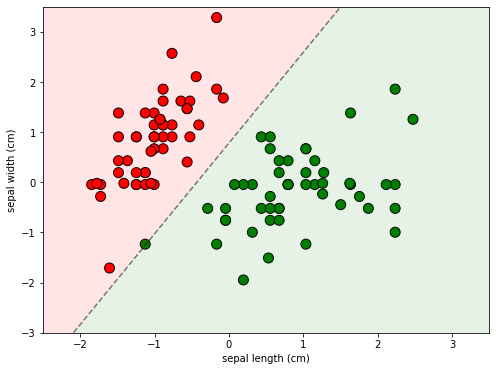
\includegraphics[width=0.7\linewidth]{bi-logistic-train-small}
	\caption{}
	\label{fig:bi-logistic-train-small}
\end{figure}

نمودار مربوط به خطا که در هر تکرار محاسبه شده است در شکل \ref{fig:bi-logistic-costs} نمایش داده شده است.

\begin{figure}[h]
	\centering
	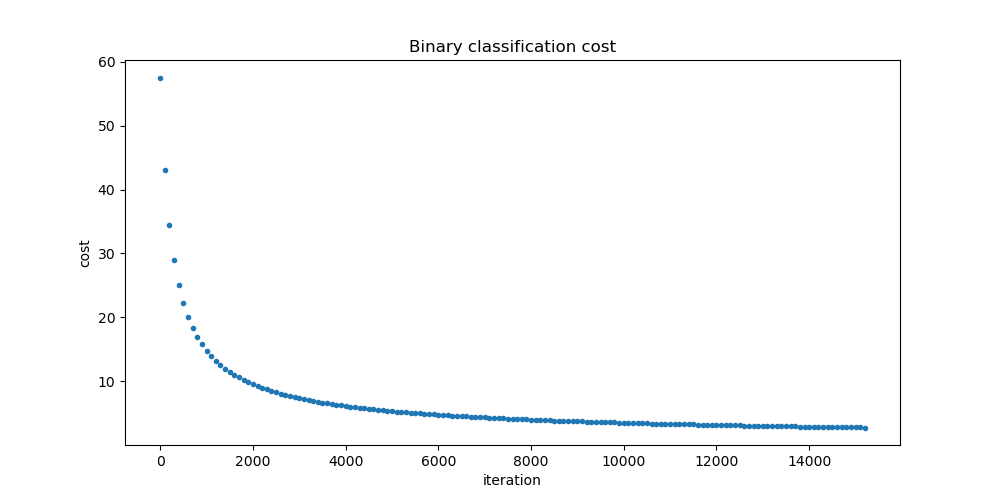
\includegraphics[width=1\linewidth]{bi-logistic-costs}
	\caption{}
	\label{fig:bi-logistic-costs}
\end{figure}
\newpage
خطای مدل بر روی داده‌های train و test در کد \ref{binary:errors} چاپ شده‌اند.

\begin{code}[h]
	\begin{latin}
		\begin{minted}{bash}
			cross-entropy (train): 0.02060000069254901
			cross-entropy (test): 0.00011377187125823006
			theta: [[ 1.84193838]
				[ 4.25519669]
				[-2.35164349]]
		\end{minted}
	\end{latin}
	\caption{خطا‌های مربوط به مدل دو کلاسه}
	\label{binary:errors}
\end{code}
\\
همچنین فرمول خط \lr{decision boundary} به صورت معادله \ref{decision-bundary} است:

\begin{equation}
	y = 1.8095 x + 0.7833
	\label{decision-bundary}
\end{equation}

\section{\textbf{\lr{Multiclass Classification}}}

\subsection{\lr{One-vs-Rest}}
این روش به تعداد کلاس‌های موجود در داده یک مدل دو کلاسه آموزش می‌دهد و یکی از مشکلات این روش نا متوازن شدن داده‌ها هنگام یادگیری است.\\
پس از آموزش مدل با ورودی‌های نمایش داده شده در کد \ref{ovr-params} مقادیر مربوط به میزان دقت هم چنین شماره‌ی تکرار همگرایی در کد \ref{ovr-accuracy} چاپ شده‌اند.
\begin{code}[h]
	\begin{latin}
		\begin{minted}{python}
			ovr = MulticlassClassifier(eta=1e-4, tol=1e-5, n_iters=1e4, solver='ovr')
			ovr.fit(df_train.iloc[:, :-1].to_numpy(), df_train.iloc[:, -1])
		\end{minted}
	\end{latin}
	\caption{ورودی‌های مدل OvR}
	\label{ovr-params}
\end{code}

\begin{code}[h]
	\begin{latin}
		\begin{minted}{bash}
			accuracy (train): 0.8416666666666667
			accuracy (test): 0.7666666666666667
			convergence iteration: 623
			theta: 
			[[-0.70711877 -0.63176098  0.74534982 -0.93384678 -0.87968063]
			[-0.70249057   0.06307685 -0.7776572   0.11260695 -0.10848047]
			[-0.64453415   0.48343572  0.09691334  0.76237581  0.9371994 ]]
		\end{minted}
	\end{latin}
	\caption{میزان دقت مدل OvR و شماره تکرار همگرایی}
	\label{ovr-accuracy}
\end{code}

نمودار مربوط به تابع هزینه در شکل \ref{fig:multi-logistic-costs} نمایش داده شده است.

\begin{figure}
	\centering
	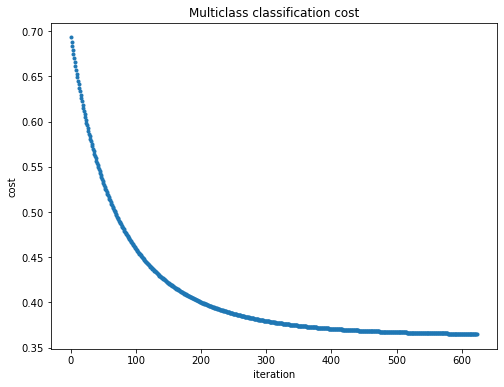
\includegraphics[width=0.8\linewidth]{multi-logistic-costs-small}
	\caption{}
	\label{fig:multi-logistic-costs}
\end{figure}


\newpage

\subsection{\lr{One-vs-One}}
در این روش به ازای هر جفت کلاس یک مدل دو کلاسه آموزش داده می‌شود و بر خلاف روش OvR از نامتوازن بودن داده‌ها رنج نمی‌برد اما با افزایش تعداد کلاس‌ها زمان یادگیری به صورت نمایی افزایش خواهد یافت.\\
ورودی های مربوط به این مدل در کد \ref{ovo-params} آمده است. همچنین مقادیر مربوط به دقت مدل در کد \ref{ovo-accuracy} نمایش داده شده است.


\begin{code}[h]
	\begin{latin}
		\begin{minted}{python}
			ovo = MulticlassClassifier(
				eta=1e-4, n_iters=1e5, solver='ovo')
			ovo.fit(df_train.iloc[:, :-1].to_numpy(), df_train.iloc[:, -1])
		\end{minted}
	\end{latin}
	\caption{ورودی‌های مدل OvO}
	\label{ovo-params}
\end{code}


\begin{code}[h]
	\begin{latin}
		\begin{minted}{bash}
			accuracy (train): 0.975
			accuracy (test): 0.8333333333333334
			theta:
			[[-3.85686431 -1.79558686  2.53491411 -3.56922839 -2.95230439]
			[-1.37635674  -1.3988      1.41402754 -2.77723175 -2.92909212]
			[ 7.48237415   0.86189624  0.97550359 -6.46540629 -6.8184238 ]]
		\end{minted}
	\end{latin}
	\caption{میزان دقت مدل OvO}
	\label{ovo-accuracy}
\end{code}

\newpage

\section{Softmax}
برای این الگوریتم تنها مقدار خواسته شده پس از آموزش مدل میزان دقت آن است که در کد \ref{softmax-accuracy} چاپ شده است.
\begin{code}[h]
	\begin{latin}
		\begin{minted}{bash}
			accuracy (train): 0.9833333333333333
			accuracy (test): 0.9333333333333333
			theta:
			[[-0.67669442, -3.01944273,  2.64580279, -5.81525285, -5.26884148],
			[ 6.42054669,  2.0871986 , -0.48711804, -2.5175024 , -2.19956475],
			[-5.74385227,  0.93224413, -2.15868475,  8.33275525,  7.46840622]]
		\end{minted}
	\end{latin}
	\caption{میزان دقت مدل softmax}
	\label{softmax-accuracy}
\end{code}

با توجه به اندازه گریری های انجام شده به خوبی مشاهده می‌شود که عملکرد الگوریتم softmax از سایر الگوریتم ها بهتر بوده است و بعد از آن الگوریتم OvO قرار دارد که عملکردی مشابه با softmax داشته. البته زمان اجرای این الگوریتم بسیار بیشتر از softmax بوده است. به دلیل آنکه تعداد classifier ها در هر دو حالت OvO و OvR با هم برابرند در نتیجه زمان اجرای دو الگوریتم با یکدیگر تفاوت چندانی ندارند و به نظر می‌رسد دلیل عملکرد ضعیف‌تر روش OvR، نامتوازن بودن تعداد داده‌های مربوط به هر کلاس در مراحل مختلف آموزش مدل است.

\end{document}

